\documentclass[11pt]{article}
\usepackage[margin=1in]{geometry}
\usepackage{setspace}\onehalfspacing
\usepackage{amsmath,amssymb}
\usepackage{graphicx,float}
\usepackage{booktabs,threeparttable}
\usepackage[authoryear,round]{natbib}
\usepackage[hidelinks]{hyperref}
\usepackage{caption}
\captionsetup{font=small,labelfont=bf}
\usepackage{enumitem}
\setlist{itemsep=2pt,topsep=4pt}
\usepackage{appendix}
\usepackage{xcolor}
\usepackage{array}
\usepackage{placeins}
\newcolumntype{L}[1]{>{\raggedright\arraybackslash}p{#1}}
\newcommand{\authornote}[1]{\textcolor{red}{[AUTHOR: #1]}}
% generated by code/40_paper.py -- do not edit
\newcommand{\accChanges}{55}
\newcommand{\accForecast}{84}
\newcommand{\accNaive}{79}
\newcommand{\accWorsenings}{54}
\newcommand{\aidAllFourCurPool}{27}
\newcommand{\aidAllFourCurPoolCi}{\textminus{}1 to 62}
\newcommand{\aidAllFourCurWithin}{4}
\newcommand{\aidAllFourCurWithinCi}{\textminus{}13 to 23}
\newcommand{\aidAllFourFcPool}{76}
\newcommand{\aidAllFourFcPoolCi}{44 to 115}
\newcommand{\aidAllFourFcWithin}{4}
\newcommand{\aidAllFourFcWithinCi}{\textminus{}11 to 22}
\newcommand{\aidAllThreeCurPool}{11}
\newcommand{\aidAllThreeCurPoolCi}{\textminus{}2 to 26}
\newcommand{\aidAllThreeCurWithin}{\textminus{}1}
\newcommand{\aidAllThreeCurWithinCi}{\textminus{}8 to 7}
\newcommand{\aidAllThreeFcPool}{26}
\newcommand{\aidAllThreeFcPoolCi}{9 to 46}
\newcommand{\aidAllThreeFcWithin}{10}
\newcommand{\aidAllThreeFcWithinCi}{3 to 19}
\newcommand{\aidFoodFourCurPool}{38}
\newcommand{\aidFoodFourCurPoolCi}{\textminus{}1 to 94}
\newcommand{\aidFoodFourCurWithin}{7}
\newcommand{\aidFoodFourCurWithinCi}{\textminus{}17 to 38}
\newcommand{\aidFoodFourFcPool}{118}
\newcommand{\aidFoodFourFcPoolCi}{67 to 184}
\newcommand{\aidFoodFourFcWithin}{4}
\newcommand{\aidFoodFourFcWithinCi}{\textminus{}21 to 38}
\newcommand{\aidFoodThreeCurPool}{20}
\newcommand{\aidFoodThreeCurPoolCi}{1 to 43}
\newcommand{\aidFoodThreeCurWithin}{\textminus{}2}
\newcommand{\aidFoodThreeCurWithinCi}{\textminus{}14 to 12}
\newcommand{\aidFoodThreeFcPool}{45}
\newcommand{\aidFoodThreeFcPoolCi}{15 to 82}
\newcommand{\aidFoodThreeFcWithin}{25}
\newcommand{\aidFoodThreeFcWithinCi}{5 to 48}
\newcommand{\amnAnyDiag}{35}
\newcommand{\amnAnyN}{1,427}
\newcommand{\amnDerCorr}{0.20}
\newcommand{\amnDerCountries}{8}
\newcommand{\amnDerN}{902}
\newcommand{\amnExpAgree}{42}
\newcommand{\amnExpCorr}{0.13}
\newcommand{\amnExpN}{600}
\newcommand{\aucEvents}{1,009}
\newcommand{\aucN}{12,776}
\newcommand{\aucRaw}{0.79}
\newcommand{\aucRawFews}{0.85}
\newcommand{\aucRawFewsPct}{85}
\newcommand{\aucRawIPC}{0.84}
\newcommand{\aucRawIPCFews}{0.86}
\newcommand{\aucRawPct}{79}
\newcommand{\bcBetaFive}{22}
\newcommand{\bcBetaFour}{10}
\newcommand{\bcBetaOne}{10}
\newcommand{\bcBetaThree}{28}
\newcommand{\bcBetaTwo}{11}
\newcommand{\bcBudget}{45}
\newcommand{\bcBudgetHigh}{65}
\newcommand{\bcBudgetLow}{35}
\newcommand{\bcCostCrisisFive}{14}
\newcommand{\bcCostCrisisFour}{22}
\newcommand{\bcCostFiveCons}{1,200}
\newcommand{\bcCostFiveMid}{570}
\newcommand{\bcCostFiveUp}{350}
\newcommand{\bcCostFourCons}{1,900}
\newcommand{\bcCostFourMid}{920}
\newcommand{\bcCostFourUp}{560}
\newcommand{\bcCostOneCons}{150,000}
\newcommand{\bcCostOneMid}{99,000}
\newcommand{\bcCostOneUp}{87,000}
\newcommand{\bcCostThreeCons}{110,000}
\newcommand{\bcCostThreeMid}{84,000}
\newcommand{\bcCostThreeUp}{120,000}
\newcommand{\bcCostTwoCons}{100,000}
\newcommand{\bcCostTwoMid}{60,000}
\newcommand{\bcCostTwoUp}{46,000}
\newcommand{\bcCrisisFive}{3.2}
\newcommand{\bcCrisisFour}{2.0}
\newcommand{\bcCrisisOne}{0.0}
\newcommand{\bcCrisisThree}{0.0}
\newcommand{\bcCrisisTwo}{0.0}
\newcommand{\bcDeathsFiveCons}{37,600}
\newcommand{\bcDeathsFiveMid}{78,300}
\newcommand{\bcDeathsFiveUp}{127,300}
\newcommand{\bcDeathsFourCons}{23,500}
\newcommand{\bcDeathsFourMid}{49,100}
\newcommand{\bcDeathsFourUp}{80,000}
\newcommand{\bcDeathsOneCons}{300}
\newcommand{\bcDeathsOneMid}{500}
\newcommand{\bcDeathsOneUp}{500}
\newcommand{\bcDeathsThreeCons}{400}
\newcommand{\bcDeathsThreeMid}{500}
\newcommand{\bcDeathsThreeUp}{400}
\newcommand{\bcDeathsTwoCons}{400}
\newcommand{\bcDeathsTwoMid}{800}
\newcommand{\bcDeathsTwoUp}{1,000}
\newcommand{\bcDistinctHi}{150,000}
\newcommand{\bcDistinctLo}{46,000}
\newcommand{\bcFlaggedAreas}{3,376}
\newcommand{\bcFlaggedRounds}{11,671}
\newcommand{\bcGrossCons}{80}
\newcommand{\bcGrossCrisis}{6.5}
\newcommand{\bcGrossMid}{168}
\newcommand{\bcGrossUp}{274}
\newcommand{\bcOneHi}{n.a.}
\newcommand{\bcOneLo}{n.a.}
\newcommand{\bcOneShareFood}{\textminus{}4.4}
\newcommand{\bcPeople}{28}
\newcommand{\bcPhaseThree}{42}
\newcommand{\bcPhaseTwo}{50}
\newcommand{\bcSfourEmerg}{25}
\newcommand{\bcShareFive}{47}
\newcommand{\bcShareFour}{29}
\newcommand{\bcShareOne}{0.3}
\newcommand{\bcShareThree}{0.3}
\newcommand{\bcShareTwo}{0.4}
\newcommand{\bcSthreeCrisis}{34}
\newcommand{\bcSthreeEmerg}{60}
\newcommand{\bcSthreeStressed}{10}
\newcommand{\bcWastingHi}{14,000}
\newcommand{\bcWastingLo}{9,000}
\newcommand{\bcWholeHi}{1,900}
\newcommand{\bcWholeHiBudgetHi}{2,800}
\newcommand{\bcWholeLo}{350}
\newcommand{\bcWholeLoBudgetLo}{270}
\newcommand{\bootOffAllFews}{0.003}
\newcommand{\bootOffAllProj}{0.014}
\newcommand{\bootOffNewFews}{0.006}
\newcommand{\bootOffNewProj}{0.006}
\newcommand{\calCdrHi}{0.25}
\newcommand{\calCdrLo}{0.07}
\newcommand{\calCdrMid}{0.15}
\newcommand{\calFamHi}{1.9}
\newcommand{\calFamLo}{0.9}
\newcommand{\calFamMid}{1.5}
\newcommand{\calGamHi}{2.5}
\newcommand{\calGamLo}{0.6}
\newcommand{\calGamMid}{1.5}
\newcommand{\caseEtAreas}{678}
\newcommand{\caseEtCurFour}{9}
\newcommand{\caseEtCurThree}{173}
\newcommand{\caseEtFcFour}{26}
\newcommand{\caseEtFlagShare}{15}
\newcommand{\caseEtFlags}{103}
\newcommand{\caseEtNextFour}{24}
\newcommand{\caseEtNextThree}{162}
\newcommand{\caseEtRain}{\textminus{}1.1}
\newcommand{\caseSoAreas}{199}
\newcommand{\caseSoCurFour}{16}
\newcommand{\caseSoCurThree}{60}
\newcommand{\caseSoFcFour}{26}
\newcommand{\caseSoFlagShare}{48}
\newcommand{\caseSoFlags}{95}
\newcommand{\caseSoNextFour}{29}
\newcommand{\caseSoNextThree}{122}
\newcommand{\caseSoRain}{\textminus{}0.8}
\newcommand{\cgBarPerDeath}{4,000}
\newcommand{\cgBudgetHi}{86}
\newcommand{\cgBudgetLo}{28}
\newcommand{\cgFiftyHi}{120}
\newcommand{\cgFiftyLo}{36}
\newcommand{\cgFortyHi}{87}
\newcommand{\cgFortyLo}{26}
\newcommand{\cgHungerHi}{28}
\newcommand{\cgHungerLo}{4}
\newcommand{\cgThirtyHi}{65}
\newcommand{\cgThirtyLo}{20}
\newcommand{\cgWholeHi}{11,000}
\newcommand{\cgWholeLo}{2,100}
\newcommand{\chCountries}{18}
\newcommand{\chFcsCorr}{0.33}
\newcommand{\chHhsCorr}{0.34}
\newcommand{\chLcsCorr}{0.15}
\newcommand{\chN}{2,805}
\newcommand{\chRcsiCorr}{0.04}
\newcommand{\contribRawCur}{0.13}
\newcommand{\contribRawCurSe}{0.02}
\newcommand{\contribRawFc}{0.13}
\newcommand{\contribRawFcSe}{0.02}
\newcommand{\contribRawIPCCur}{0.12}
\newcommand{\contribRawIPCCurSe}{0.02}
\newcommand{\contribRawIPCFc}{0.08}
\newcommand{\contribRawIPCFcSe}{0.02}
\newcommand{\covCountries}{70}
\newcommand{\covPfour}{82}
\newcommand{\covPost}{\textminus{}0.002}
\newcommand{\covPostSe}{0.002}
\newcommand{\covPre}{\textminus{}0.009}
\newcommand{\covPreSe}{0.018}
\newcommand{\covPthree}{69}
\newcommand{\csAreaMonths}{209,404}
\newcommand{\csAreas}{16,684}
\newcommand{\csCountries}{37}
\newcommand{\dCostBudgetHi}{220,000}
\newcommand{\dCostBudgetLo}{36,000}
\newcommand{\dCostCrisisHi}{2,700}
\newcommand{\dCostCrisisLo}{1,600}
\newcommand{\dCostEmergHi}{1,100}
\newcommand{\dCostEmergLo}{400}
\newcommand{\dCostWastHi}{910,000}
\newcommand{\dCostWastLo}{190,000}
\newcommand{\dCostWastMax}{2,800,000}
\newcommand{\dCostWastMin}{120,000}
\newcommand{\dCrisisHi}{28,000}
\newcommand{\dCrisisLo}{17,000}
\newcommand{\dDeathsHi}{970}
\newcommand{\dDeathsLo}{290}
\newcommand{\dEmergHi}{110,000}
\newcommand{\dEmergLo}{41,000}
\newcommand{\dShareHi}{0.4}
\newcommand{\dShareLo}{0.3}
\newcommand{\dWastHi}{240}
\newcommand{\dWastLo}{50}
\newcommand{\envBeta}{28}
\newcommand{\envPmHi}{9.6}
\newcommand{\envPmLo}{4.2}
\newcommand{\envShareIpc}{7}
\newcommand{\envSharePosRaw}{16}
\newcommand{\envShareRaw}{9}
\newcommand{\envUsdHi}{370}
\newcommand{\envUsdLo}{274}
\newcommand{\famCame}{0}
\newcommand{\famEpisodes}{5}
\newcommand{\famFlag}{50}
\newcommand{\famForecastFive}{0}
\newcommand{\famForecastFour}{3}
\newcommand{\famLower}{50}
\newcommand{\famMapped}{103}
\newcommand{\famMappedUnits}{98}
\newcommand{\famMissed}{100}
\newcommand{\famNoFlag}{0}
\newcommand{\famRiskLeadSd}{12}
\newcommand{\famRiskLeadSo}{6}
\newcommand{\famRiskSd}{June 2023}
\newcommand{\famRiskSo}{January 2011}
\newcommand{\famWarn}{6}
\newcommand{\famWarnUnits}{6}
\newcommand{\fcPredictsWorsening}{56}
\newcommand{\fdwCorr}{0.40}
\newcommand{\fdwN}{389}
\newcommand{\fdwNfews}{332}
\newcommand{\fdwSlope}{3.3}
\newcommand{\fdwSlopeSe}{1.1}
\newcommand{\flagIpc}{0.15}
\newcommand{\flagIpcP}{0.26}
\newcommand{\flagIpcPlacebo}{0.22}
\newcommand{\flagIpcSe}{0.09}
\newcommand{\flagOwn}{0.09}
\newcommand{\flagOwnP}{0.43}
\newcommand{\flagOwnPlacebo}{0.20}
\newcommand{\flagOwnSe}{0.07}
\newcommand{\fsAll}{1,248}
\newcommand{\fsAucFc}{0.47}
\newcommand{\fsAucLag}{0.75}
\newcommand{\fsChRtwoFc}{\textminus{}0.01}
\newcommand{\fsChRtwoLag}{0.27}
\newcommand{\fsCorrAfter}{0.09}
\newcommand{\fsCorrFc}{0.10}
\newcommand{\fsCorrLag}{0.66}
\newcommand{\fsCrit}{33}
\newcommand{\fsDfc}{0.6}
\newcommand{\fsDfcSe}{0.4}
\newcommand{\fsFcOnLag}{0.09}
\newcommand{\fsFcOnLagSe}{0.05}
\newcommand{\fsFcsCorr}{0.41}
\newcommand{\fsFcsCorrArea}{0.15}
\newcommand{\fsFcsCorrCty}{0.27}
\newcommand{\fsFcsFour}{46}
\newcommand{\fsFcsHighUnder}{5}
\newcommand{\fsFcsLowOver}{71}
\newcommand{\fsFcsN}{3,500}
\newcommand{\fsFcsOne}{28}
\newcommand{\fsFcsSdOne}{15}
\newcommand{\fsFcsThree}{47}
\newcommand{\fsFcsTwo}{35}
\newcommand{\fsFoodAreas}{478}
\newcommand{\fsFoodCountries}{29}
\newcommand{\fsGam}{13}
\newcommand{\fsGamFour}{15}
\newcommand{\fsGamThree}{13}
\newcommand{\fsGamTwo}{13}
\newcommand{\fsLead}{3}
\newcommand{\fsMortFc}{\textminus{}0.07}
\newcommand{\fsMortLag}{0.20}
\newcommand{\fsMortN}{323}
\newcommand{\fsN}{329}
\newcommand{\fsRcsiCorr}{0.35}
\newcommand{\fsRcsiCorrArea}{0.25}
\newcommand{\fsRcsiCorrCty}{0.25}
\newcommand{\fsRcsiFour}{45}
\newcommand{\fsRcsiHighUnder}{4}
\newcommand{\fsRcsiLowOver}{78}
\newcommand{\fsRcsiN}{2,484}
\newcommand{\fsRcsiOne}{33}
\newcommand{\fsRcsiSdOne}{19}
\newcommand{\fsRcsiThree}{49}
\newcommand{\fsRcsiTwo}{35}
\newcommand{\fsRtwoBoth}{0.41}
\newcommand{\fsRtwoFc}{\textminus{}0.10}
\newcommand{\fsRtwoLag}{0.42}
\newcommand{\fsSeasons}{28}
\newcommand{\fsZones}{29}
\newcommand{\ftsShareFews}{56}
\newcommand{\ftsUsFoodShare}{52}
\newcommand{\grfcFewsSourcePthree}{6}
\newcommand{\hetAllDiff}{\textminus{}0.49}
\newcommand{\hetAllDiffSe}{0.59}
\newcommand{\hetAllHigh}{8}
\newcommand{\hetAllLow}{13}
\newcommand{\hetFoodDiff}{\textminus{}1.80}
\newcommand{\hetFoodDiffSe}{1.31}
\newcommand{\hetFoodHigh}{16}
\newcommand{\hetFoodLow}{39}
\newcommand{\hetShareHigh}{32}
\newcommand{\infoFcEsc}{11}
\newcommand{\infoFcNew}{6}
\newcommand{\infoMapEsc}{10}
\newcommand{\infoMapNew}{18}
\newcommand{\ipcCgHi}{1,100}
\newcommand{\ipcCgLo}{270}
\newcommand{\ipcDeathsHi}{12,000}
\newcommand{\ipcDeathsLo}{3,100}
\newcommand{\ipcDistinctHi}{15,000}
\newcommand{\ipcDistinctLo}{3,700}
\newcommand{\ipcGrossCons}{121}
\newcommand{\ipcGrossMid}{562}
\newcommand{\ipcGrossUp}{820}
\newcommand{\ipcWholeHi}{790}
\newcommand{\ipcWholeLo}{100}
\newcommand{\maskInter}{0.009}
\newcommand{\maskInterSe}{0.028}
\newcommand{\maskMappedHigh}{0.49}
\newcommand{\maskMappedLow}{0.50}
\newcommand{\maskNeedHigh}{0.49}
\newcommand{\maskNeedLow}{0.51}
\newcommand{\moneyRawAllBase}{3}
\newcommand{\moneyRawAllBaseCi}{\textminus{}10 to 18}
\newcommand{\moneyRawAllContrib}{12}
\newcommand{\moneyRawAllContribCi}{4 to 21}
\newcommand{\moneyRawFoodBase}{10}
\newcommand{\moneyRawFoodBaseCi}{\textminus{}17 to 46}
\newcommand{\moneyRawFoodContrib}{33}
\newcommand{\moneyRawFoodContribCi}{11 to 59}
\newcommand{\moneyRawIPCAllBase}{7}
\newcommand{\moneyRawIPCAllBaseCi}{\textminus{}5 to 21}
\newcommand{\moneyRawIPCAllContrib}{11}
\newcommand{\moneyRawIPCAllContribCi}{3 to 19}
\newcommand{\moneyRawIPCFoodBase}{18}
\newcommand{\moneyRawIPCFoodBaseCi}{\textminus{}8 to 51}
\newcommand{\moneyRawIPCFoodContrib}{31}
\newcommand{\moneyRawIPCFoodContribCi}{9 to 57}
\newcommand{\needEarly}{\textminus{}6}
\newcommand{\needEarlySe}{5}
\newcommand{\needHeld}{55}
\newcommand{\needHeldSteady}{78}
\newcommand{\needOnsets}{2,338}
\newcommand{\ngSlope}{2.7}
\newcommand{\ngSlopeSe}{0.8}
\newcommand{\nsCritDown}{0.2}
\newcommand{\nsCritDownSe}{4.4}
\newcommand{\nsCritN}{1,015}
\newcommand{\nsCritUp}{11.9}
\newcommand{\nsCritUpSe}{4.6}
\newcommand{\nsDown}{\textminus{}0.7}
\newcommand{\nsDownSe}{3.0}
\newcommand{\nsEsc}{6.4}
\newcommand{\nsEscBase}{8.7}
\newcommand{\nsEscSe}{2.6}
\newcommand{\nsForecast}{15}
\newcommand{\nsNone}{6}
\newcommand{\nsOkDown}{\textminus{}8.6}
\newcommand{\nsOkDownSe}{3.7}
\newcommand{\nsOkN}{271}
\newcommand{\nsOkUp}{14.8}
\newcommand{\nsOkUpSe}{4.7}
\newcommand{\nsShare}{3.5}
\newcommand{\nsStressBase}{11}
\newcommand{\nsStressDown}{\textminus{}1.1}
\newcommand{\nsStressDownSe}{1.1}
\newcommand{\nsStressN}{848}
\newcommand{\nsStressUp}{7.5}
\newcommand{\nsStressUpSe}{2.5}
\newcommand{\nsUnforecast}{25}
\newcommand{\nsUp}{8.8}
\newcommand{\nsUpBase}{10}
\newcommand{\nsUpSe}{3.1}
\newcommand{\obAvgCore}{44}
\newcommand{\obAvgLong}{37}
\newcommand{\obMin}{22}
\newcommand{\obPeak}{63}
\newcommand{\obPillarOne}{139}
\newcommand{\offCoefAllFews}{0.18}
\newcommand{\offCoefAllProj}{0.06}
\newcommand{\offCoefNewFews}{0.15}
\newcommand{\offCoefNewProj}{0.05}
\newcommand{\offCountries}{12}
\newcommand{\offCountriesAll}{14}
\newcommand{\offFaEither}{15}
\newcommand{\offFaFews}{7}
\newcommand{\offFaOfficial}{12}
\newcommand{\offHitEither}{55}
\newcommand{\offHitFews}{37}
\newcommand{\offHitOfficial}{42}
\newcommand{\offHitOnlyFews}{12}
\newcommand{\offN}{4,128}
\newcommand{\offNall}{6,683}
\newcommand{\offNew}{227}
\newcommand{\offYears}{2014--2025}
\newcommand{\outAug}{6}
\newcommand{\outBefore}{32}
\newcommand{\outOct}{21}
\newcommand{\panelAreaRounds}{190,131}
\newcommand{\panelAreas}{16,053}
\newcommand{\panelCountries}{28}
\newcommand{\prBoth}{51}
\newcommand{\prFewsOnly}{16}
\newcommand{\prMarketsFews}{881}
\newcommand{\prNone}{11}
\newcommand{\prShareNonWfp}{77}
\newcommand{\prWfpOnly}{22}
\newcommand{\predBaseSd}{0.22}
\newcommand{\predBaseSdWithin}{0.10}
\newcommand{\predContribSd}{0.15}
\newcommand{\predContribSdWithin}{0.15}
\newcommand{\predCountrySeason}{61}
\newcommand{\predShocksWithin}{5}
\newcommand{\pvEscBase}{0.711}
\newcommand{\pvEscBoth}{0.719}
\newcommand{\pvEscFc}{0.823}
\newcommand{\pvEscFews}{0.723}
\newcommand{\pvEscRaw}{0.714}
\newcommand{\pvEscRawBoth}{0.714}
\newcommand{\pvEscRawMap}{0.817}
\newcommand{\pvEscWfp}{0.738}
\newcommand{\pvNewBase}{0.844}
\newcommand{\pvNewBoth}{0.846}
\newcommand{\pvNewFc}{0.900}
\newcommand{\pvNewFews}{0.845}
\newcommand{\pvNewRaw}{0.725}
\newcommand{\pvNewRawBoth}{0.727}
\newcommand{\pvNewRawMap}{0.901}
\newcommand{\pvNewWfp}{0.844}
\newcommand{\shareChanges}{21}
\newcommand{\shareWithIndependent}{25}
\newcommand{\shockRsq}{1.7}
\newcommand{\shockRsqRain}{0.06}
\newcommand{\spCdrFour}{0.31}
\newcommand{\spCdrOne}{0.32}
\newcommand{\spCdrSlope}{0.00}
\newcommand{\spCdrSlopeIpc}{0.17}
\newcommand{\spCdrSlopeIpcSe}{0.05}
\newcommand{\spCdrSlopeSe}{0.04}
\newcommand{\spCdrThree}{0.40}
\newcommand{\spCdrTwo}{0.45}
\newcommand{\spCorr}{0.32}
\newcommand{\spGamFour}{18}
\newcommand{\spGamOne}{9}
\newcommand{\spGamThree}{11}
\newcommand{\spGamTwo}{10}
\newcommand{\spN}{246}
\newcommand{\spNfews}{167}
\newcommand{\spNround}{90}
\newcommand{\spSlope}{1.8}
\newcommand{\spSlopeSe}{0.5}
\newcommand{\subSdAidShare}{14}
\newcommand{\subSdAny}{\textminus{}0.03}
\newcommand{\subSdAnyPct}{\textminus{}3}
\newcommand{\subSdAnySe}{0.03}
\newcommand{\subSdBase}{1.06}
\newcommand{\subSdBaseSe}{0.65}
\newcommand{\subSdContrib}{0.02}
\newcommand{\subSdContribSe}{0.29}
\newcommand{\subSdDistricts}{192}
\newcommand{\subSdFc}{\textminus{}0.32}
\newcommand{\subSdFcSe}{0.38}
\newcommand{\subSdFlagAid}{\textminus{}0.002}
\newcommand{\subSdFlagAidSe}{0.001}
\newcommand{\subSdFlagPersist}{0.72}
\newcommand{\subSdFlagPersistSe}{0.04}
\newcommand{\subSdFlagPres}{0.010}
\newcommand{\subSdFlagPresSe}{0.003}
\newcommand{\subSdFlagReach}{0.000}
\newcommand{\subSdFlagReachPc}{0.000}
\newcommand{\subSdFlagReachPcSe}{0.000}
\newcommand{\subSdFlagReachSe}{0.002}
\newcommand{\subSdIvF}{10}
\newcommand{\subSdPeriods}{18}
\newcommand{\subSdPlac}{0.20}
\newcommand{\subSdPlacSe}{0.28}
\newcommand{\subSdPres}{0.39}
\newcommand{\subSdPresSe}{0.40}
\newcommand{\subSdReach}{\textminus{}0.20}
\newcommand{\subSdReachSe}{0.38}
\newcommand{\subSoAidShare}{12}
\newcommand{\subSoAny}{0.08}
\newcommand{\subSoAnyPct}{8}
\newcommand{\subSoAnySe}{0.03}
\newcommand{\subSoBase}{2.82}
\newcommand{\subSoBaseSe}{0.68}
\newcommand{\subSoContrib}{\textminus{}0.01}
\newcommand{\subSoContribSe}{0.32}
\newcommand{\subSoDistricts}{74}
\newcommand{\subSoFc}{1.10}
\newcommand{\subSoFcSe}{0.37}
\newcommand{\subSoFlagAid}{0.004}
\newcommand{\subSoFlagAidSe}{0.002}
\newcommand{\subSoFlagMean}{20}
\newcommand{\subSoFlagPersist}{0.28}
\newcommand{\subSoFlagPersistSe}{0.02}
\newcommand{\subSoFlagPres}{0.009}
\newcommand{\subSoFlagPresSe}{0.002}
\newcommand{\subSoFlagReach}{0.012}
\newcommand{\subSoFlagReachPc}{0.096}
\newcommand{\subSoFlagReachPcSe}{0.016}
\newcommand{\subSoFlagReachSd}{17}
\newcommand{\subSoFlagReachSe}{0.021}
\newcommand{\subSoIvF}{4}
\newcommand{\subSoPeriods}{33}
\newcommand{\subSoPlac}{0.72}
\newcommand{\subSoPlacSe}{0.25}
\newcommand{\subSoPres}{0.20}
\newcommand{\subSoPresSe}{0.33}
\newcommand{\subSoReach}{1.69}
\newcommand{\subSoReachSe}{0.81}
\newcommand{\svCritShare}{86}
\newcommand{\svET}{52}
\newcommand{\svEmergET}{67}
\newcommand{\svEmergSD}{14}
\newcommand{\svEmergSO}{54}
\newcommand{\svGamFive}{39}
\newcommand{\svGamFour}{31}
\newcommand{\svGamThree}{22}
\newcommand{\svGamTwo}{19}
\newcommand{\svPopET}{17}
\newcommand{\svPopSD}{16}
\newcommand{\svPopSO}{36}
\newcommand{\svSD}{23}
\newcommand{\svSO}{188}
\newcommand{\svTotal}{263}
\newcommand{\svvCostHi}{650,000}
\newcommand{\svvCostLo}{27,000}
\newcommand{\svvCostMid}{100,000}
\newcommand{\svvDeaths}{2}
\newcommand{\svvFc}{73}
\newcommand{\svvOracle}{75}
\newcommand{\svvRand}{48}
\newcommand{\svvRateFc}{46}
\newcommand{\svvRateHi}{5,100}
\newcommand{\svvRateLo}{210}
\newcommand{\svvRateMid}{820}
\newcommand{\svvRateSurvey}{53}
\newcommand{\svvRound}{240,000}
\newcommand{\svvSurvey}{73}
\newcommand{\svvZones}{12}
\newcommand{\tIIanyEmergency}{57}
\newcommand{\tIIcontrolEmergency}{1.3}
\newcommand{\tIIcrisisOnly}{39}
\newcommand{\tIIearlyCrisis}{42}
\newcommand{\tIIearlyCrisisPlus}{89}
\newcommand{\tIIearlyEmergency}{47}
\newcommand{\tIIearlyMiss}{53}
\newcommand{\tIIearlyStressed}{11}
\newcommand{\tIIfromCrisis}{85}
\newcommand{\tIIleadeight}{22}
\newcommand{\tIIleadfour}{42}
\newcommand{\tIIleadfourCrisis}{95}
\newcommand{\tIIleadone}{63}
\newcommand{\tIInoWarning}{4}
\newcommand{\tIIonsets}{1,562}
\newcommand{\tIbetter}{3}
\newcommand{\tIcame}{46}
\newcommand{\tIcountries}{9}
\newcommand{\tIfailFlagShare}{56}
\newcommand{\tIfailed}{54}
\newcommand{\tIflagShareOfCrisis}{60}
\newcommand{\tIflagUnwarnedCrisis}{12}
\newcommand{\tIflagged}{30}
\newcommand{\tIflaggedAlreadyFlagged}{48}
\newcommand{\tIgenuine}{23}
\newcommand{\tIunflagged}{20}
\newcommand{\tIwarnings}{4,084}
\newcommand{\txtAccess}{7}
\newcommand{\txtAidDown}{6}
\newcommand{\txtAucMap}{0.60}
\newcommand{\txtAucMapText}{0.59}
\newcommand{\txtAucNeed}{0.71}
\newcommand{\txtAucNeedText}{0.73}
\newcommand{\txtEscEvents}{744}
\newcommand{\txtEscFcFour}{32}
\newcommand{\txtEscN}{8,564}
\newcommand{\txtMatch}{91}
\newcommand{\txtMatchN}{322}
\newcommand{\txtOutlooks}{135}
\newcommand{\txtReports}{502}
\newcommand{\vmAreas}{1,803}
\newcommand{\vmCountries}{24}
\newcommand{\vmCover}{32}
\newcommand{\vmCoverHi}{36}
\newcommand{\vmCoverLo}{29}
\newcommand{\vmFewsCountries}{37}
\newcommand{\vmFoodAll}{4.0}
\newcommand{\vmFoodSample}{2.5}
\newcommand{\vmHalfAid}{54}
\newcommand{\vmHalfAidAll}{88}
\newcommand{\vmHalfCostPm}{11}
\newcommand{\vmHalfFews}{59}
\newcommand{\vmHalfGain}{2.4}
\newcommand{\vmHalfGainAll}{3.9}
\newcommand{\vmHalfOracle}{70}
\newcommand{\vmHalfOracleGain}{17}
\newcommand{\vmHalfPctMore}{4}
\newcommand{\vmHalfPub}{56}
\newcommand{\vmHalfRatio}{1.2}
\newcommand{\vmHalfRatioAll}{2.0}
\newcommand{\vmHalfRatioAllHi}{2.8}
\newcommand{\vmHalfRatioAllLo}{1.2}
\newcommand{\vmHalfShareNeed}{0.7}
\newcommand{\vmNeed}{346}
\newcommand{\vmPerfAid}{21}
\newcommand{\vmPerfAidAll}{34}
\newcommand{\vmPerfCostPm}{30}
\newcommand{\vmPerfFews}{81}
\newcommand{\vmPerfGain}{0.9}
\newcommand{\vmPerfGainAll}{1.5}
\newcommand{\vmPerfOracle}{100}
\newcommand{\vmPerfOracleGain}{5}
\newcommand{\vmPerfPctMore}{1}
\newcommand{\vmPerfPub}{80}
\newcommand{\vmPerfRatio}{0.5}
\newcommand{\vmPerfRatioAll}{0.8}
\newcommand{\vmPerfRatioAllHi}{1.1}
\newcommand{\vmPerfRatioAllLo}{0.5}
\newcommand{\vmPerfShareNeed}{0.3}
\newcommand{\vmRandAid}{59}
\newcommand{\vmRandAidAll}{95}
\newcommand{\vmRandCostPm}{11}
\newcommand{\vmRandFews}{35}
\newcommand{\vmRandGain}{2.6}
\newcommand{\vmRandGainAll}{4.2}
\newcommand{\vmRandOracle}{45}
\newcommand{\vmRandOracleGain}{20}
\newcommand{\vmRandPctMore}{8}
\newcommand{\vmRandPub}{32}
\newcommand{\vmRandRatio}{1.3}
\newcommand{\vmRandRatioAll}{2.1}
\newcommand{\vmRandRatioAllHi}{3.0}
\newcommand{\vmRandRatioAllLo}{1.3}
\newcommand{\vmRandShareNeed}{0.8}
\newcommand{\vmScale}{1.6}
\newcommand{\vmYears}{2013--2024}
\newcommand{\voiBase}{5,651}
\newcommand{\voiCostFull}{1,900}
\newcommand{\voiCostHalf}{1,700}
\newcommand{\voiCostHiFull}{2,900}
\newcommand{\voiCostHiHalf}{2,500}
\newcommand{\voiCostHiZero}{2,100}
\newcommand{\voiCostLoFull}{970}
\newcommand{\voiCostLoHalf}{830}
\newcommand{\voiCostLoZero}{700}
\newcommand{\voiCostZero}{1,400}
\newcommand{\voiGainFull}{122}
\newcommand{\voiGainHalf}{142}
\newcommand{\voiGainZero}{168}
\newcommand{\voiOracleDeaths}{6,914}
\newcommand{\voiOracleFull}{27}
\newcommand{\voiOracleHalf}{18}
\newcommand{\voiOracleZero}{13}
\newcommand{\voiPop}{5,671}
\newcommand{\voiRangeHi}{2,200}
\newcommand{\voiRangeLo}{1,200}
\newcommand{\voiSamShare}{16}
\newcommand{\voiSeasons}{26}
\newcommand{\voiZones}{12}
\newcommand{\wholeHi}{1,900}
\newcommand{\wholeLo}{350}
\newcommand{\wzCdrZone}{0.12}
\newcommand{\wzCdrZoneMap}{0.12}
\newcommand{\wzCdrZoneMapSe}{0.03}
\newcommand{\wzCdrZoneSe}{0.03}
\newcommand{\wzCdrZoneSeason}{0.08}
\newcommand{\wzCdrZoneSeasonMap}{0.09}
\newcommand{\wzCdrZoneSeasonMapSe}{0.03}
\newcommand{\wzCdrZoneSeasonSe}{0.04}
\newcommand{\wzGamZone}{0.8}
\newcommand{\wzGamZoneMap}{1.2}
\newcommand{\wzGamZoneMapSe}{0.5}
\newcommand{\wzGamZoneSe}{0.3}
\newcommand{\wzGamZoneSeason}{0.5}
\newcommand{\wzGamZoneSeasonMap}{0.6}
\newcommand{\wzGamZoneSeasonMapSe}{0.6}
\newcommand{\wzGamZoneSeasonSe}{0.3}
\newcommand{\wzSlopeFig}{0.5}
\newcommand{\wzUfiveZone}{0.25}
\newcommand{\wzUfiveZoneMap}{0.23}
\newcommand{\wzUfiveZoneMapSe}{0.04}
\newcommand{\wzUfiveZoneSe}{0.07}
\newcommand{\wzUfiveZoneSeason}{0.14}
\newcommand{\wzUfiveZoneSeasonMap}{0.08}
\newcommand{\wzUfiveZoneSeasonMapSe}{0.04}
\newcommand{\wzUfiveZoneSeasonSe}{0.08}


\title{What Do Food Insecurity Phases Measure? IPC Classifications Against Household and Nutrition Surveys}
\author{Working draft (companion to ``How Much Does Early Warning Improve Famine Response?'')}
\date{October 2026 \\ \small Material moved from the FEWS NET evaluation; not yet edited as a standalone paper}
\begin{document}
\maketitle

\noindent\authornote{This draft collects the sections on what IPC and FEWS NET phases measure, on surveys, and on the value of surveys, moved out of the FEWS NET evaluation. Cross-references to that paper appear as ``??''.}

\section{What do FEWS NET's phases measure?}\label{sec:phase}

So far we have scored FEWS NET's phases against later phases. Before valuing them, we ask what a phase captures on the ground. FEWS NET's phases, like the IPC's, are meant to measure acute food insecurity: whether households can eat enough, and what they give up to do so. We test that first, with household surveys run by others. Evaluations often go further and read phases as signals of malnutrition and death, using the IPC's reference bands for each phase; we test that too, more briefly, with the details in Appendix~\ref{app:phase}.

\subsection{Food consumption and coping}

By design, the IPC's acute food insecurity phase summarizes household food consumption and the strategies households use to cope with shortfalls. We test that directly with survey measures of the same indicators that were not produced by the IPC or FEWS NET: WFP's household food security surveys and its monthly phone monitoring, compiled by the European Commission's Joint Research Centre \citep{machefer2025hfid}, together with WFP's monitoring files, by region, matched to FEWS NET's map for the same area and month. The data cover \fsFoodAreas{} areas in \fsFoodCountries{} countries between 2011 and 2024. We use two indicators: the share of households with poor or borderline food consumption, and the share using severe coping strategies (a reduced coping strategies index of 19 or more). These are independent of the classifications in the sense that the IPC and FEWS NET did not collect them, though analysts may have seen them.

Phases track these measures, but loosely (Figures~\ref{fig:phfcs} and~\ref{fig:phrcsi}). The share of households with poor or borderline food consumption averages \fsFcsOne{}, \fsFcsTwo{}, \fsFcsThree{} and \fsFcsFour{} percent in areas FEWS NET mapped in Phases 1, 2, 3 and 4 or worse; the share coping severely averages \fsRcsiOne{}, \fsRcsiTwo{}, \fsRcsiThree{} and \fsRcsiFour{} percent. The correlations with FEWS NET's phase are \fsFcsCorr{} and \fsRcsiCorr{} across all areas, \fsFcsCorrCty{} and \fsRcsiCorrCty{} within countries, and \fsFcsCorrArea{} and \fsRcsiCorrArea{} within an area over time. The spread within each phase is wide. The IPC classifies an area in Crisis or worse when at least 20 percent of its households are in Crisis or worse, and its reference table places borderline food consumption, and a coping index of 19 or more, at Crisis. By that rule, \fsFcsLowOver{} percent of areas FEWS NET mapped in Phases 1 or 2 had too many households with poor or borderline consumption for their phase, and \fsRcsiLowOver{} percent had too many coping severely; only \fsFcsHighUnder{} and \fsRcsiHighUnder{} percent of areas mapped in Crisis or worse had too few. The indicators are consistent with the classification in Crisis areas, and much worse than it in areas classified as Minimal or Stressed.

The classification is not a formula applied to these indicators. For 2021--2023 the Cadre Harmonis\'e publishes the household indicators its analysts weighed, for \chN{} area-analyses in \chCountries{} countries. Even these correlate only loosely with the phase the same analysts assigned: \chFcsCorr{} for poor or borderline food consumption, \chHhsCorr{} for moderate or severe household hunger, \chLcsCorr{} for crisis livelihood coping and \chRcsiCorr{} for severe consumption coping. A phase is a judgment that converges several kinds of evidence, with consensus and adjustment for context. Its link to any single measured outcome is correspondingly loose: moderate for food consumption and coping, weak for child malnutrition, and close to nothing for mortality.

\begin{figure}[p]
\centering
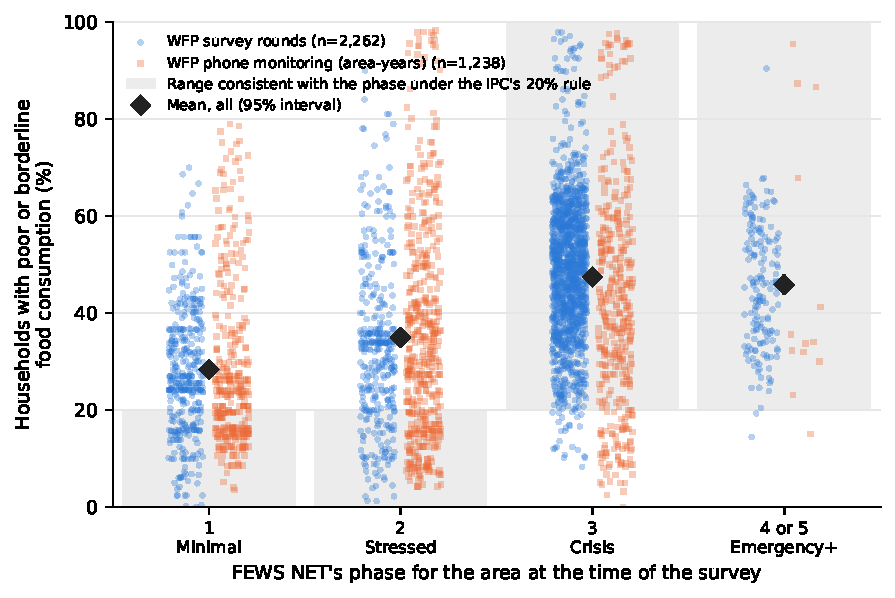
\includegraphics[width=0.9\textwidth]{figures/fig9g_phase_fcs.pdf}
\caption{Household food consumption by FEWS NET phase. Each point is one area in one survey round (blue) or one area-year of WFP's monthly phone monitoring (orange): the share of households with poor or borderline food consumption scores, against the phase FEWS NET's map gave the area at the time (mean over the FEWS NET units in the area, rounded; points jittered). Data: WFP, compiled in the Joint Research Centre's harmonized food insecurity dataset and WFP's monitoring files, by region, 2011--2024. Grey boxes: the range consistent with each phase under the IPC's rule that an area is in a phase when at least 20 percent of its households are in that phase or worse, with borderline consumption counted as Crisis and poor consumption as Emergency or worse; below 20 percent for Phases 1 and 2, at least 20 percent for Crisis or worse (this indicator cannot separate Crisis from Emergency). Diamonds: means with 95 percent intervals.}\label{fig:phfcs}
\end{figure}

\begin{figure}[p]
\centering
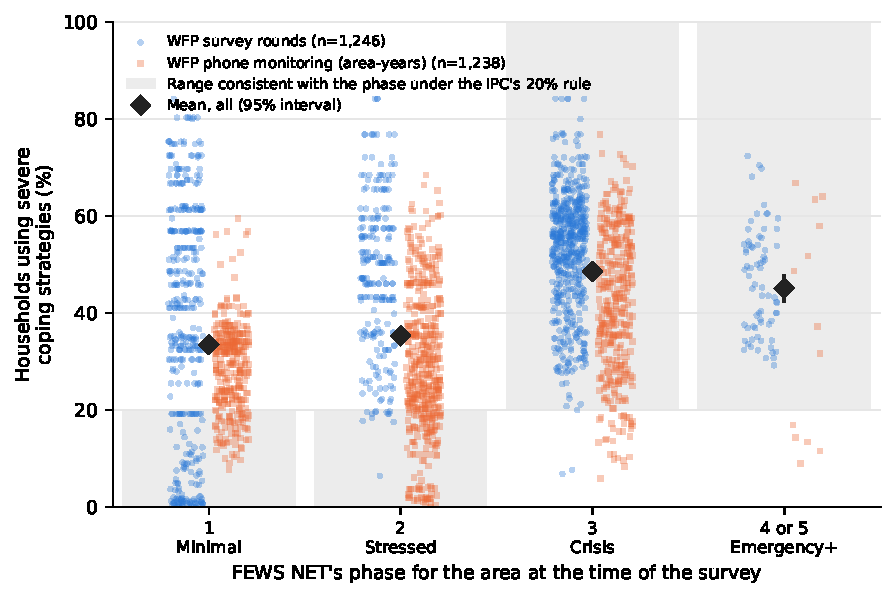
\includegraphics[width=0.9\textwidth]{figures/fig9h_phase_rcsi.pdf}
\caption{Household coping by FEWS NET phase. As Figure~\ref{fig:phfcs}, for the share of households using severe consumption coping strategies (reduced coping strategies index of 19 or more, which the IPC's reference table places at Crisis or worse). Grey boxes: the range consistent with each phase under the IPC's 20 percent rule.}\label{fig:phrcsi}
\end{figure}

\subsection{Malnutrition and mortality}

The IPC ties each phase to a band of acute malnutrition among children under five (below 5, 5--10, 10--15, 15--30 and above 30 percent) and of crude death rates (below 0.5 deaths per 10,000 people per day in Phases 1 and 2, 0.5--1 in Crisis, 1--2 in Emergency and above 2 in Famine) \citep{IPC2021manual,ipcreftable}. The bands were not derived from food insecurity data; they descend from 1980s and 1990s benchmarks for refugee camps \citep{youngjaspars2009}, and the IPC itself notes that food insecurity and acute malnutrition often diverge \citep{ipc2016amn,ipc2024linkages}. We know of no study that systematically tests the bands against survey-measured outcomes across areas.

Measured outcomes do not follow them. In Somalia, where FSNAU surveys rural zones on a fixed schedule twice a year, mean acute malnutrition was \fsGamTwo{}, \fsGamThree{} and \fsGamFour{} percent in zones FEWS NET forecast to be Stressed, in Crisis, and in Emergency or worse (Figure~\ref{fig:phgam}); the correlation with FEWS NET's forecast is \fsCorrFc{}, against \fsCorrLag{} with the zone's own survey six months earlier. Within a zone, one phase worse than usual goes with about \wzGamZone{} more points of acute malnutrition and \wzCdrZone{} more deaths per 10,000 per day (Figure~\ref{fig:within}), where the bands imply 5--10 points and 0.45--0.75 deaths. Surveys elsewhere show a steeper gradient for malnutrition, about \spSlope{}--\fdwSlope{} points per phase, and none for crude death rates (Figure~\ref{fig:phcdr}); the IPC's own malnutrition classifications agree with its food insecurity classifications for only \amnAnyDiag{} percent of areas; and the excess deaths estimated in Somalia's 2017 and 2022 droughts imply about 0.15--0.2 deaths per 10,000 per day for each person in Crisis or worse. A phase of food insecurity is a weak guide to malnutrition and a poor guide to mortality. That is why we value FEWS NET in Section~\ref{sec:bcr} in the unit it is designed to forecast, people kept out of food insecurity, and convert to lives only as a heavily qualified extension.

\begin{figure}[p]
\centering
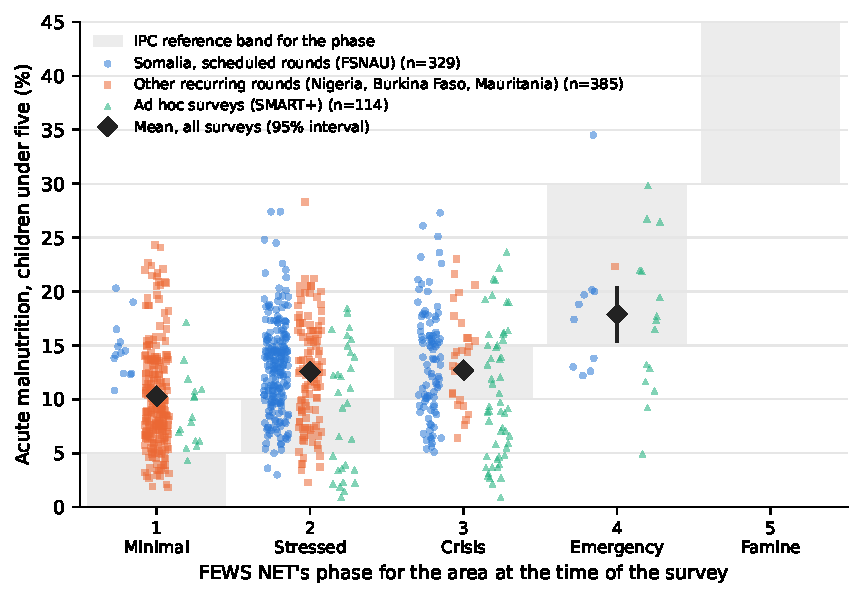
\includegraphics[width=0.9\textwidth]{figures/fig9a_phase_gam.pdf}
\caption{Measured acute malnutrition by FEWS NET phase. Each point is one survey: global acute malnutrition (weight-for-height) among children under five, against the phase FEWS NET's map gave the area at the time of the survey (rounded mean over the FEWS NET units in the survey area; points jittered). Grey boxes: the IPC reference band for each phase. Blue: Somalia's scheduled FSNAU rounds, rural zones, 2011--2024. Orange: other recurring national or sub-national rounds (Nigeria's UNICEF rounds, 2023--26; Burkina Faso and Mauritania national rounds, 2003--18). Green: ad hoc surveys in the SMART+ dashboard, 2022--26. Diamonds: mean of all surveys in the phase, with 95 percent intervals.}\label{fig:phgam}
\end{figure}

\begin{figure}[p]
\centering
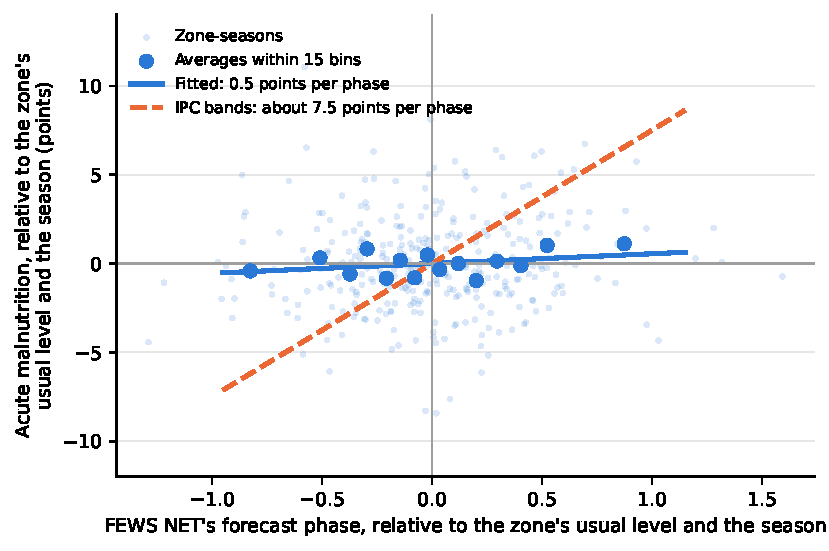
\includegraphics[width=0.82\textwidth]{figures/fig9c_within_zone.pdf}
\caption{Within zones: when FEWS NET forecasts a Somali zone to be worse than usual, is its measured malnutrition worse than usual? Both variables are measured relative to the zone's own average and the season's average across zones (zone and season effects removed). Light points: \fsN{} zone-seasons; dark points: averages within 15 equal-sized bins of the forecast. Solid line: fitted slope. Dashed line: the slope implied by the IPC reference bands, roughly the average of the 5- and 10-point steps between band midpoints.}\label{fig:within}
\end{figure}

\begin{figure}[p]
\centering
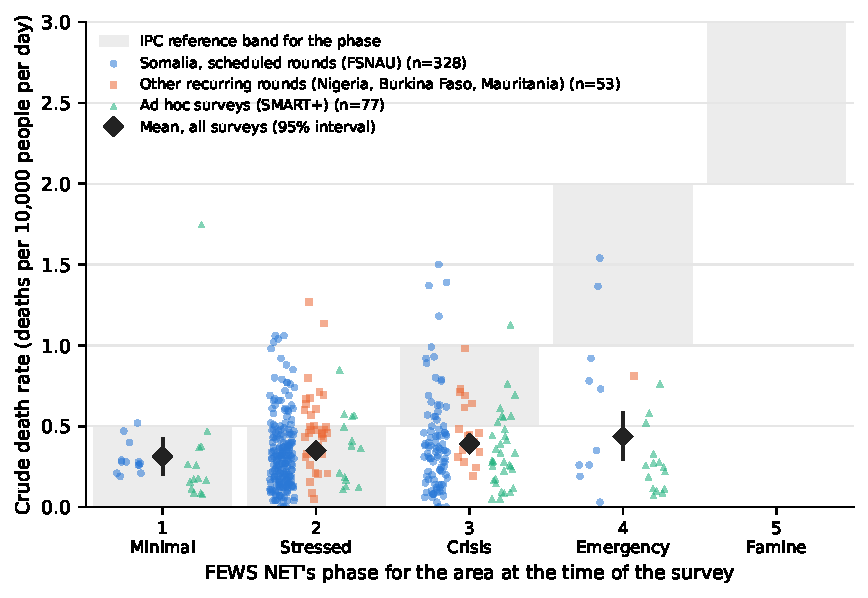
\includegraphics[width=0.9\textwidth]{figures/fig9b_phase_cdr.pdf}
\caption{Measured crude death rates by FEWS NET phase. As Figure~\ref{fig:phgam}, for crude death rates (deaths per 10,000 people per day), in surveys that measured mortality. Grey boxes: the IPC reference band for each phase.}\label{fig:phcdr}
\end{figure}


\FloatBarrier
\section{Surveys and FEWS NET's maps}\label{sec:pieces}


The reports do contain something the maps do not: the results of nutrition and mortality surveys, which measure child malnutrition and death rather than the household food insecurity that FEWS NET's phases classify. These are mostly standardized SMART surveys run by UNICEF, NGOs and national partners, and in Somalia by the FAO-managed Food Security and Nutrition Analysis Unit. We extracted \svTotal{} distinct survey results (\svSO{} in Somalia, \svET{} in Ethiopia and \svSD{} in Sudan). They measure outcomes independently of any phase classification. Mean acute malnutrition among children under five rises with FEWS NET's phase at the time of the survey: \svGamTwo{} percent in Stressed areas, \svGamThree{} percent in Crisis, \svGamFour{} percent in Emergency and \svGamFive{} percent in Famine. The reports quote surveys selectively, and \svCritShare{} percent of those quoted show acute malnutrition of 15 percent or more. So these results cannot score FEWS NET's accuracy, but they show its phases track measured malnutrition.

Survey coverage is uneven. Among area-rounds that FEWS NET mapped as Emergency, the reports quote a survey from the previous 12 months for \svEmergET{} percent in Ethiopia, \svEmergSO{} percent in Somalia and \svEmergSD{} percent in Sudan. These are lower bounds, since the reports do not quote every survey.

New surveys move the maps, and only upward. In \nsShare{} percent of area-rounds, a survey was carried out between FEWS NET's forecast and its next map. When one was, the next map was worse than the forecast \nsUp{} percentage points more often (standard error \nsUpSe{}, against a base rate of \nsUpBase{} percent). This comparison is within country and round, holds the forecast fixed, and controls for everything the reports said about the area when the forecast was made. The next map was no more likely to be better than forecast (\nsDown{} points, standard error \nsDownSe{}). Among areas in Crisis, a new survey raised the chance of moving to Emergency by \nsEsc{} points (standard error \nsEscSe{}) from a base of \nsEscBase{} percent. A survey preceded \nsUnforecast{} percent of the escalations FEWS NET had not forecast, \nsForecast{} percent of those it had, and \nsNone{} percent of the cases in Crisis that did not escalate.

Three readings could explain this. Surveys may reveal deterioration that the forecast missed. The IPC's rules may cap classifications without survey evidence, so that a survey can unlock a higher phase but its absence rarely pulls one down. Or surveys may be sent where people on the ground already suspect trouble, for reasons the reports do not state. Two checks favor the third reading. First, the rules do not explain it. The IPC requires nutrition and mortality evidence to classify Famine, and weighs it heavily for Emergency, but not for Crisis. Yet among areas forecast to be Stressed or better, a new survey raised the chance that the next map showed Crisis or worse by \nsStressUp{} percentage points (standard error \nsStressUpSe{}, base rate \nsStressBase{} percent). Second, what the survey found matters little. Surveys showing acute malnutrition below 15 percent (\nsOkN{} area-rounds) raised the chance of a worse map by \nsOkUp{} points (standard error \nsOkUpSe{}), about as much as surveys showing 15 percent or more (\nsCritUp{}, standard error \nsCritUpSe{}). If surveys moved the maps through their content, reassuring results would pull them down. Instead they made a better-than-forecast map less likely, not more (\nsOkDown{} points, standard error \nsOkDownSe{}).

So the decision to survey is itself the signal. Agencies send survey teams where conditions are slipping, and FEWS NET's next map moves with them. This tells us two things. First, the people who commission surveys know something FEWS NET's forecasts do not yet reflect. A record of where surveys are planned and why could serve as an early warning in its own right. Second, comparing places with and without surveys cannot show what better survey coverage would add to forecasts, because surveys are not placed at random. That question needs surveys whose timing is fixed in advance, such as scheduled seasonal assessments, so that their results, not the decision to collect them, can be scored. Section~\ref{sec:phase} uses Somalia's scheduled surveys to do this.

\begin{figure}[t]
\centering
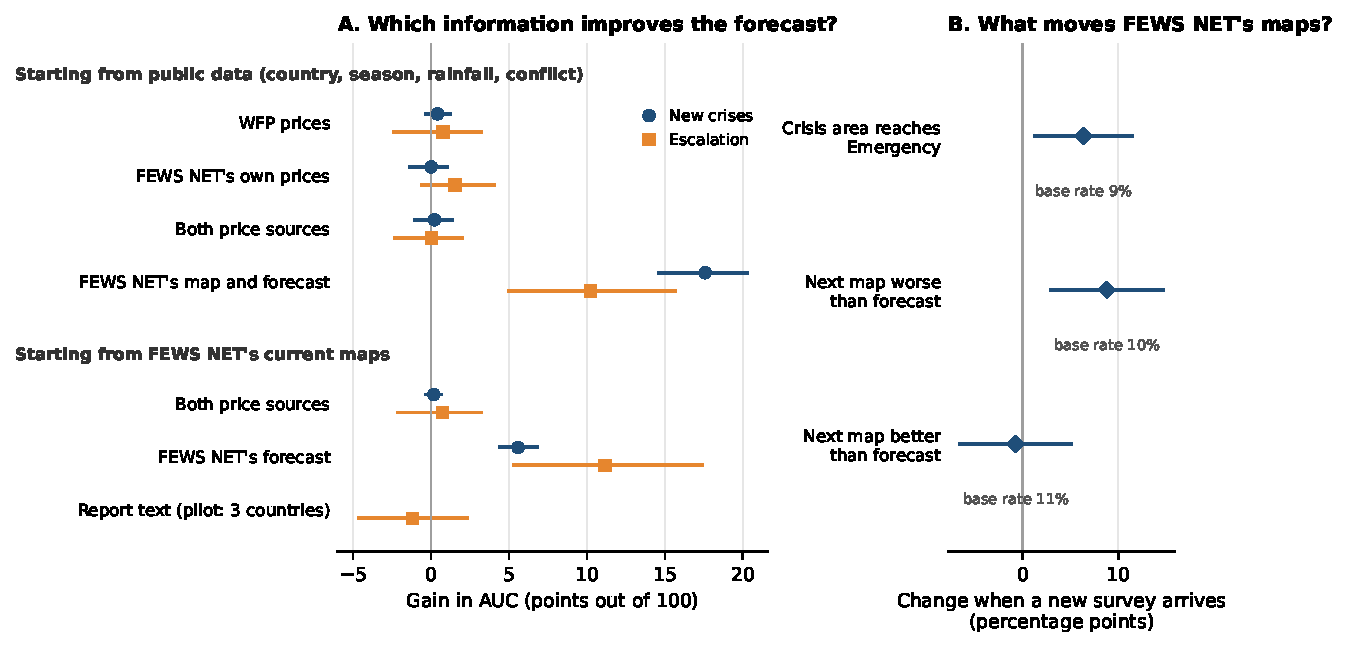
\includegraphics[width=\textwidth]{figures/fig8_information.pdf}
\caption{Which information improves forecasts of food crises? Panel A: gain in the cross-fitted AUC from adding each source of information, for areas tipping into Crisis or worse at the next FEWS NET map (circles) and for areas in Crisis escalating to Emergency or worse (squares), FEWS NET areas 2011--2024. Public data: country, calendar month, forecast horizon, rainfall (CHIRPS) and political violence (ACLED). Prices: 3- and 12-month changes in retail staple prices at the nearest market within 150 km, from WFP or from FEWS NET's own price monitoring and the government systems it compiles. Report text: features extracted from FEWS NET's written reports, Somalia, Ethiopia and Sudan only. Lines are 95 percent intervals from resampling country-years. Panel B: change in the probability of each outcome on the next map when a nutrition or mortality survey is carried out between FEWS NET's forecast and that map, Somalia, Ethiopia and Sudan, with country-by-round fixed effects and controls for the forecast and for everything the reports said about the area at the time; 95 percent intervals clustered by region.}\label{fig:information}
\end{figure}

\FloatBarrier
\section{Would paying for surveys pay off?}\label{sec:surveys}

This section turns from FEWS NET to a different product. Nutrition and mortality surveys measure acute malnutrition and death, not the food insecurity that FEWS NET and the IPC are designed to classify, so the outcomes here are lives rather than person-months of food insecurity. We include them because Section~\ref{sec:phase} shows that phases of food insecurity say little about malnutrition and death, and because a funder deciding what to pay for may want both.

If FEWS NET as a whole looks below the bar in lives saved, would more surveys look better? Surveys of acute malnutrition and mortality cost about \$15,000--21,000 for each area estimated in sub-Saharan Africa, and up to \$30,000 in harder settings \citep{unicef_aah2016smart,daher2018smart}. Somalia's scheduled programme surveys about \svvZones{} rural zones a season, plus towns and displaced settlements. For surveys to save lives, a chain of links must hold:
\begin{enumerate}
  \item more surveys give better information about where children are malnourished and dying;
  \item that information makes warnings better, earlier, or simply louder;
  \item better warnings move more aid, or move it to better places;
  \item that aid reduces malnutrition and death.
\end{enumerate}
The evidence on each link is uneven.

\paragraph{1. Information.} Strong. In Somalia, last season's survey predicts this season's acute malnutrition far better than FEWS NET's forecast (Section~\ref{sec:phase}). No other source we examined substitutes for it, and models that try to predict malnutrition without surveys have performed poorly \citep{checchi2022malnut}.

\paragraph{2. Warnings.} Weak, through FEWS NET. FEWS NET's forecasts barely respond to survey results: a zone whose last survey showed 10 more points of acute malnutrition is forecast \fsFcOnLag{} of a phase worse (standard error \fsFcOnLagSe{}). Ad hoc surveys move FEWS NET's maps upward whatever they find (Section~\ref{sec:pieces}), which looks more like added alarm than added accuracy. FEWS NET's phases are about food insecurity, and survey results about malnutrition do not translate into them.

\paragraph{3. Aid.} Mostly outside FEWS NET. Money follows FEWS NET's forecasts (Section~\ref{sec:money}), but surveys hardly shape those forecasts. Survey results reach aid more directly: nutrition programmes size their caseloads and supplies from survey prevalence, multiplying the number of children by the measured rate and a correction for new cases \citep{isanaka2021icf,bongassie2021afg}. How far donors follow such assessments is less clear \citep{olin2014sida}.

\paragraph{4. Lives.} Strong, for treatment. Treating severe acute malnutrition in the community is among the best-evidenced interventions in crises, at roughly \$4,000--7,000 per death averted when we apply GiveWell's inputs for two well-run programmes \citep{givewell2024cmam,givewell2024taimaka}. But programmes reach a minority of cases; average coverage across 21 countries was 38 percent \citep{rogers2015coverage}.

\paragraph{A coarse targeting rule.} A first, crude test asks whether surveys help a programme choose which half of the zones to serve each season. They barely do: choosing by predicted caseload, the survey-based choice covers \svvSurvey{} percent of the season's malnourished children and the forecast-based choice \svvFc{} percent, because where malnourished children are depends mostly on where children are. But a yes-or-no choice of zones wastes most of what surveys tell a planner.

\paragraph{If treatment followed surveys.} The links that hold most firmly are the first and the last: surveys measure malnutrition, and treating it saves lives. What is missing is evidence that treatment follows surveys. So we ask the counterfactual directly: if a treatment programme used survey results as well as it could, what would one round of surveys be worth?

We model a planner in Somalia who, each season, has a fixed number of treatment places for acutely malnourished children in the \voiZones{} rural zones FSNAU surveys, and spends them to avert as many deaths as possible given what it can see. Each zone has two kinds of case. Severe acute malnutrition, about \voiSamShare{} percent of cases, carries an untreated one-year mortality of about 10 percent, which treatment cuts by about 70 percent; moderate acute malnutrition carries about 4 percent, cut by about 40 percent \citep{givewell2024cmam}. Caseloads are zone population times the share under five times measured prevalence times the standard correction for new cases \citep{isanaka2021icf}, and at most 80 percent of a zone's cases can be reached. The planner sends places first where it predicts the most deaths averted per place, up to its predicted reachable caseload in each zone. Places sent to a zone with fewer cases than predicted are stranded; in two variants, half or all of them can be moved once the true caseload is known. The planner predicts each zone's severe and moderate prevalence in one of three ways: from the national average, from FEWS NET's forecast phase, or from the zone's previous survey; and we compare these with perfect foresight. All predictions are made out of sample.

Survey-based planning saves more lives at every realistic budget (Figure~\ref{fig:voi}). With places for 38 percent of the caseload, the average coverage of treatment programmes, a planner using FEWS NET's forecast averts about \voiBase{} deaths a season; one using the previous survey averts \voiGainZero{} more if stranded places cannot be moved, \voiGainHalf{} more if half can, and \voiGainFull{} more if all can. That is \voiOracleZero{}--\voiOracleFull{} percent of the gain perfect foresight would bring. A planner who knows only population does about as well as one using FEWS NET's forecast. Most of the survey's value comes from knowing where severe cases are, so that places go to the children most likely to die; moving stranded supplies cannot undo that kind of misallocation. A round of surveys in these zones costs about \$\svvRound{}, so the extra deaths averted cost about \$\voiCostZero{}--\voiCostFull{} each (\$\voiCostLoZero{}--\voiCostHiFull{} across survey costs and redeployment), and \$\voiRangeLo{}--\voiRangeHi{} across budgets of 20--50 percent of the caseload. The value disappears only at the extremes, when the budget is so small that it is spent on severe cases anywhere, or so large that nearly every case can be reached, and stranded supplies can all be moved.

This is an upper bound in one sense and a lower bound in another. It assumes treatment programmes act on survey results as well as they could, which is the point of the exercise but not current practice. It uses GiveWell's mortality inputs before its adjustments, and Somalia's surveyed zones only. But it values surveys only for placing treatment within a fixed budget. It gives them no credit for sizing that budget, for detecting famine conditions, or for evaluation.

\begin{figure}[t]
\centering
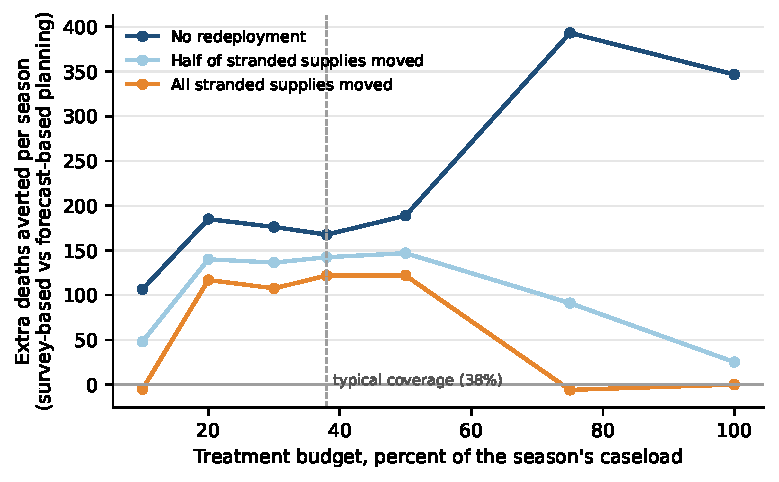
\includegraphics[width=0.72\textwidth]{figures/fig10_voi.pdf}
\caption{If treatment followed surveys: extra deaths averted per season in Somalia when a planner places treatment using each zone's previous scheduled survey rather than FEWS NET's forecast, by the size of the treatment budget: the number of treatment places as a share of all acutely malnourished children in the surveyed zones that season (horizontal axis). \voiZones{} surveyed rural zones per season over \voiSeasons{} seasons. The planner allocates treatment places to severe and moderate acute malnutrition by zone to maximize predicted deaths averted; places sent to zones with fewer cases than predicted are stranded, and none, half or all of them can be moved once caseloads are known. Mortality and treatment effects from GiveWell's inputs; caseloads from measured prevalence, population and the standard incidence correction.}\label{fig:voi}
\end{figure}

\paragraph{What this implies.} The case for paying for more surveys does not rest on better FEWS NET warnings: FEWS NET's phases do not carry the information that matters for treatment, and its forecasts barely respond to survey results. It rests on what surveys can do for the response directly. If treatment programmes placed their resources by survey results, a round of Somalia's surveys would avert deaths at roughly \$\voiRangeLo{}--\voiRangeHi{} each, in the range of the most cost-effective charities and far cheaper than FEWS NET's distinctive information. Whether that value is realized depends on whether funders and programmes act on survey results, which in turn depends on surveys being regular, timely and public. Surveys also have value we do not count: sizing the response, seeing famine-level conditions directly, and knowing afterwards whether a response worked \citep{kenny2026humanitarian}.

\FloatBarrier
\appendix
\section{Malnutrition and mortality by phase: details}\label{app:phase}

\subsection{Why the bands may not hold}

The bands were not derived from food insecurity data. They descend from 1980s and 1990s benchmarks for refugee camps: a doubling of a baseline crude death rate of about 0.44, and camp-based relations between wasting and mortality \citep{youngjaspars2009}. When the IPC created a separate scale for acute malnutrition in 2016, it noted that food insecurity and acute malnutrition do not always match, in either direction \citep{ipc2016amn}. Acute malnutrition depends on disease, water, sanitation and care as well as food. A meta-analysis of household studies finds that food insecurity predicts stunting and underweight but not wasting \citep{moradi2019}, and studies in Chad, Darfur, South Sudan and Niger find wasting hotspots that do not coincide with food-insecurity hotspots \citep{youngmarshak2017,luc2023chad}. In Somalia, models that forecast acute malnutrition lean mainly on its own past values \citep{checchi2022malnut,reusken2025}, and a FEWS NET causal analysis in Niger found household food insecurity not independently associated with wasting \citep{mcdonald2017nca}.

\subsection{Method}

We use three kinds of evidence. First, survey measurements matched to FEWS NET's phase for the same area and time. For a survey of area $a$ in season $t$, with measured outcome $y_{at}$ (acute malnutrition, or a crude or under-five death rate) and FEWS NET phase $P_{at}$ (its forecast for the survey month, or its map), we estimate
\begin{equation*}
y_{at} = \beta P_{at} + \mu_a + \lambda_t + \varepsilon_{at}.
\end{equation*}
Without the area effects $\mu_a$, $\beta$ compares different areas: are areas in worse phases worse off? With them, it compares the same area over time: when an area is one phase worse than usual, how much worse are its outcomes? The second is what the benefit-cost calculation needs, since it asks what happens when aid holds a given area one phase better. The season effects $\lambda_t$ remove shocks common to the country in a season. We also score FEWS NET's forecast as a predictor of $y_{at}$ out of sample, leaving out one season at a time, against the simplest alternative: the area's own measurement in the previous round.

Which surveys are used matters. Surveys sent where trouble is suspected will overstate the link between phase and outcome, because they are fielded where both are bad (Section~\ref{sec:pieces}). So we rely mainly on scheduled surveys, fielded on a fixed calendar whatever the conditions, and treat ad hoc surveys as an upper bound. Second, we compare the IPC's two scales, for acute food insecurity and for acute malnutrition, where both classify the same area. Third, we compare the excess deaths estimated in documented crises with the number of people in Crisis or worse.

\subsection{Somalia's scheduled surveys}

Somalia's Food Security and Nutrition Analysis Unit (FSNAU), managed by FAO, surveys the country's rural livelihood zones, towns and displaced settlements twice a year, after the Gu and Deyr rains, on a fixed calendar. We assembled all \fsAll{} survey results it published from late 2010 to 2026, from its results portal and its technical reports. We kept the rural SMART surveys run by FSNAU itself and matched each surveyed zone to FEWS NET's mapping units by livelihood zone and region. That leaves \fsN{} zone-seasons in \fsZones{} zones over \fsSeasons{} seasons with FEWS NET's forecast, its current map and the zone's result from the previous round. Mean acute malnutrition was \fsGam{} percent, and \fsCrit{} percent of zone-seasons were at or above the critical level of 15 percent. Two caveats apply. Insecure zones of south-central Somalia, notably Juba, South Gedo and parts of Bakool and Hiran, were often skipped or assessed only by arm-circumference screening, so the worst-hit areas are under-represented. And FSNAU's analysts work alongside FEWS NET's, though the survey measurements are independent of the classifications.

Across zones, FEWS NET's phases do not track measured malnutrition (Figure~\ref{fig:phgam}, blue points). Mean acute malnutrition was \fsGamTwo{} percent in zones FEWS NET forecast to be Stressed or better, \fsGamThree{} percent in zones forecast to be in Crisis and \fsGamFour{} percent in zones forecast to be in Emergency or worse. The correlation between FEWS NET's forecast, issued a median of \fsLead{} months ahead, and the measured rate is \fsCorrFc{}. The correlation with FEWS NET's map published just after the survey, which could draw on its results, is \fsCorrAfter{}. The zone's own result six months earlier correlates \fsCorrLag{} with this round's (Figure~\ref{fig:persist}). Out of sample, the previous survey explains \fsRtwoLag{} of the variance in acute malnutrition, and FEWS NET's forecast explains none ($R^2$ of \fsRtwoFc{}); adding the forecast to the previous survey does not help (\fsRtwoBoth{}). For predicting whether a zone reaches the critical level, the AUC is \fsAucLag{} with the previous survey and \fsAucFc{} with FEWS NET's forecast. The same holds for under-five death rates: out-of-sample $R^2$ of \fsMortLag{} for the previous survey and \fsMortFc{} for the forecast.

Within zones there is a gradient, but a small one (Figure~\ref{fig:within}). When FEWS NET forecast a zone to be one phase worse than usual, its acute malnutrition was \wzGamZone{} points higher (standard error \wzGamZoneSe{}), or \wzGamZoneSeason{} points (\wzGamZoneSeasonSe{}) with season effects. Its crude death rate was \wzCdrZone{} deaths per 10,000 per day higher (\wzCdrZoneSe{}), or \wzCdrZoneSeason{} (\wzCdrZoneSeasonSe{}) with season effects, and its under-five death rate \wzUfiveZone{} (\wzUfiveZoneSe{}) or \wzUfiveZoneSeason{} (\wzUfiveZoneSeasonSe{}) higher. Using FEWS NET's map after the survey instead of its forecast gives similar estimates. At their midpoints, the IPC bands imply 5 points of acute malnutrition and 0.45 deaths per 10,000 per day for a step from Stressed to Crisis, and 10 points and 0.75 deaths for a step from Crisis to Emergency. 
The estimates may be biased down: the phase of a survey zone averages several FEWS NET units, which adds noise, and the worst-hit zones are under-surveyed. They are consistent with \citet{reusken2025}, who find that the official share of a district's population in Phase 3 or worse helps predict its acute malnutrition: a link exists, but it is far weaker than the bands imply.


\begin{figure}[H]
\centering
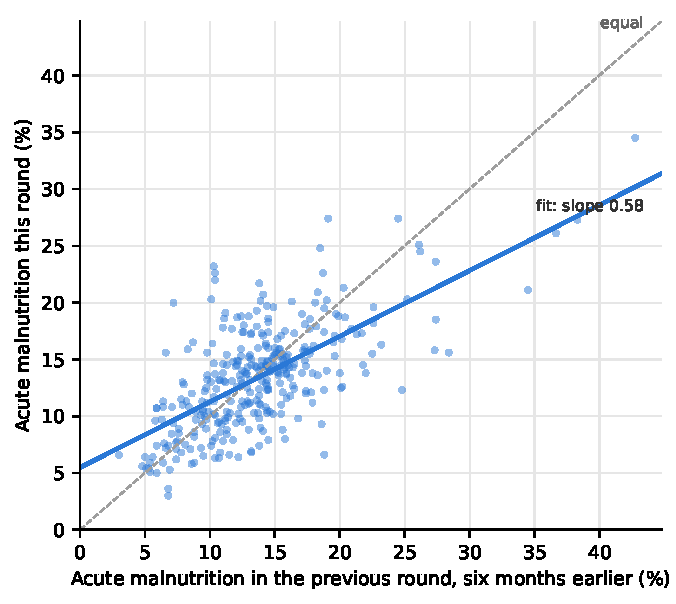
\includegraphics[width=0.62\textwidth]{figures/fig9d_persistence.pdf}
\caption{Somalia's scheduled surveys: acute malnutrition in a rural zone this round against the same zone six months earlier, \fsN{} zone-seasons, 2011--2024. Solid line: least-squares fit; dashed line: equality.}\label{fig:persist}
\end{figure}

\subsection{Other countries}

We repeated the comparison with two open sources. The SMART+ dashboard run by Action Against Hunger and UNICEF holds \spN{} survey results from 2022 to 2026, mostly from Nigeria, Ethiopia and Mozambique, \spNfews{} of which fall in FEWS NET's maps; \spNround{} come from Nigeria's recurring UNICEF survey rounds and the rest are ad hoc. FEWS NET's data warehouse holds \fdwN{} results from national survey rounds in Burkina Faso and Mauritania, 2003--2018.\footnote{The warehouse lists several thousand Ethiopian survey results as public, but does not return their values.} The gradient is steeper than in Somalia but still well below the bands (Figure~\ref{fig:phgam}, orange and green points). In SMART+, mean acute malnutrition was \spGamOne{}, \spGamTwo{}, \spGamThree{} and \spGamFour{} percent in areas FEWS NET mapped in Phases 1, 2, 3 and 4 or worse (correlation \spCorr{}); the jump at Phase 4 comes mostly from a dozen ad hoc surveys in Ethiopia. With country-by-year effects, one phase goes with \spSlope{} points of acute malnutrition (standard error \spSlopeSe{}). Nigeria's recurring rounds give \ngSlope{} points (\ngSlopeSe{}) per Cadre Harmonis\'e phase, and the Burkina Faso and Mauritania rounds \fdwSlope{} (\fdwSlopeSe{}) per FEWS NET phase. Crude death rates do not rise with FEWS NET's phase at all (Figure~\ref{fig:phcdr}): \spCdrOne{}, \spCdrTwo{}, \spCdrThree{} and \spCdrFour{} deaths per 10,000 per day across the four groups (slope \spCdrSlope{}, standard error \spCdrSlopeSe{}). Against the official IPC or Cadre Harmonis\'e phase, they rise by \spCdrSlopeIpc{} per phase (\spCdrSlopeIpcSe{}).


The IPC's own two scales tell the same story (Figure~\ref{fig:amn}). Where an area has both an acute food insecurity phase and an acute malnutrition phase for the same period, the two correlate \amnExpCorr{} and agree exactly in \amnExpAgree{} percent of \amnExpN{} areas in the Democratic Republic of Congo, Nigeria and South Sudan. Classifying acute malnutrition from published prevalence in \amnDerCountries{} countries gives a correlation of \amnDerCorr{} across \amnDerN{} areas. Pooling both, the two scales put an area in the same phase only \amnAnyDiag{} percent of the time across \amnAnyN{} areas, and areas the food insecurity scale calls Crisis are spread almost evenly across all four malnutrition phases.

\begin{figure}[H]
\centering
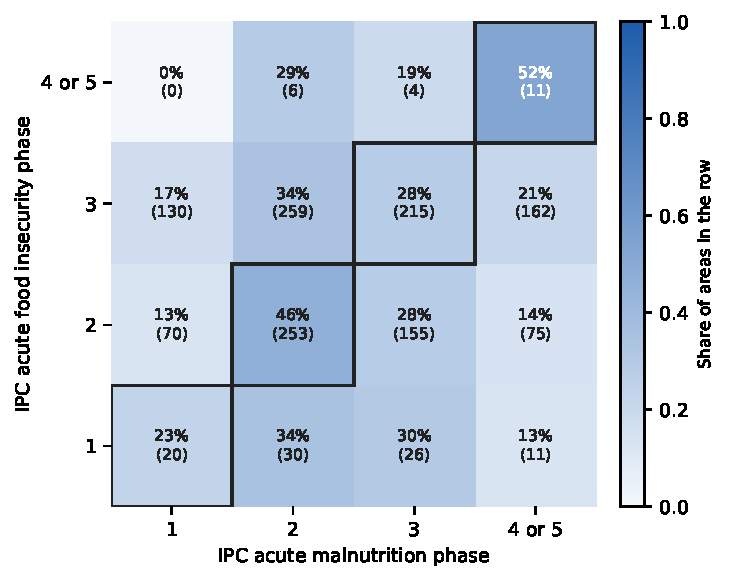
\includegraphics[width=0.66\textwidth]{figures/fig9e_afi_amn.pdf}
\caption{The IPC's two scales for the same areas. Rows: the IPC acute food insecurity phase of the area; columns: its acute malnutrition phase for the same period (published by the IPC, or classified from published acute malnutrition prevalence using the IPC's thresholds). Each cell gives the share of the row and the number of areas; outlined cells are where the two scales agree. \amnAnyN{} areas in Afghanistan, the Central African Republic, Cameroon, the Democratic Republic of Congo, Mali, Mozambique, Nigeria, Somalia and South Sudan, 2021--2026 (years vary by country).}\label{fig:amn}
\end{figure}

\subsection{Excess deaths in documented crises}

The most direct evidence on mortality comes from crises whose death tolls have been estimated. Dividing estimated excess deaths by the number of people in Crisis or worse gives an excess death rate per person in Phase 3 or worse of roughly 0.15--0.2 per 10,000 per day in Somalia's 2017--18 and 2022 droughts \citep{warsame2023,lshtm2023somalia,ouchtar2026}, about 0.9 in northeast Nigeria in 2016--19 \citep{checchi2023nigeria}, and 1.1--1.9 in the 2010--12 Somalia famine, which met a late response \citep{checchi2013}. Figure~\ref{fig:excess} sets these against the IPC's Crisis band. Measured crude death rates in areas reviewed for famine since 2017 have mostly been between 0.3 and 1.9, below the IPC's famine threshold of 2 \citep{ipcfrc2022somaliadec,ipcfrc2024sudandec}. Arithmetic with the IPC bands would have predicted roughly two to five times the excess deaths estimated for Somalia in 2022.

\begin{figure}[H]
\centering
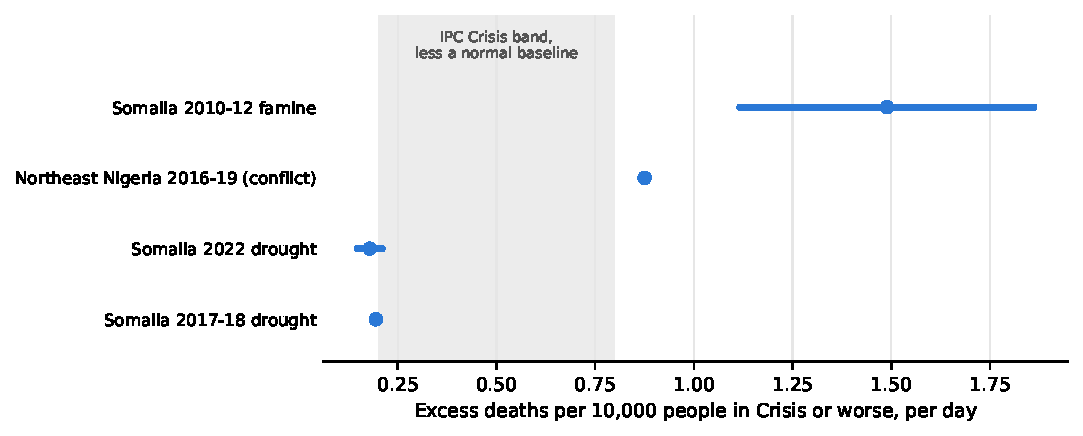
\includegraphics[width=0.85\textwidth]{figures/fig9f_excess_deaths.pdf}
\caption{Excess deaths in documented crises, per person in Crisis or worse. Estimated excess deaths divided by the number of people classified in IPC or Cadre Harmonis\'e Phase 3 or worse and the length of the crisis; ranges reflect ranges in the death toll and in the Phase 3+ population. Grey band: the IPC Crisis band for crude death rates (0.5--1 per 10,000 per day) less a normal baseline of 0.2--0.3. Sources: \citet{warsame2023,lshtm2023somalia,checchi2023nigeria,checchi2013}.}\label{fig:excess}
\end{figure}


\newpage
\bibliographystyle{chicago}
\bibliography{references}
\end{document}
